% Fig. 1 v5: instruction -> prior lane vs AG3S lane on one SafeLIBERO episode.
% Source: paper/figures/fig01_teaser/v5/fig01_v5.pdf (+ fig01_v5.json). Scripts: fig1_v4_assets.py, cvpr_v5_fig1_compose.py.
\begin{minipage}{\textwidth}
\centering
\captionsetup{type=figure,hypcap=false}
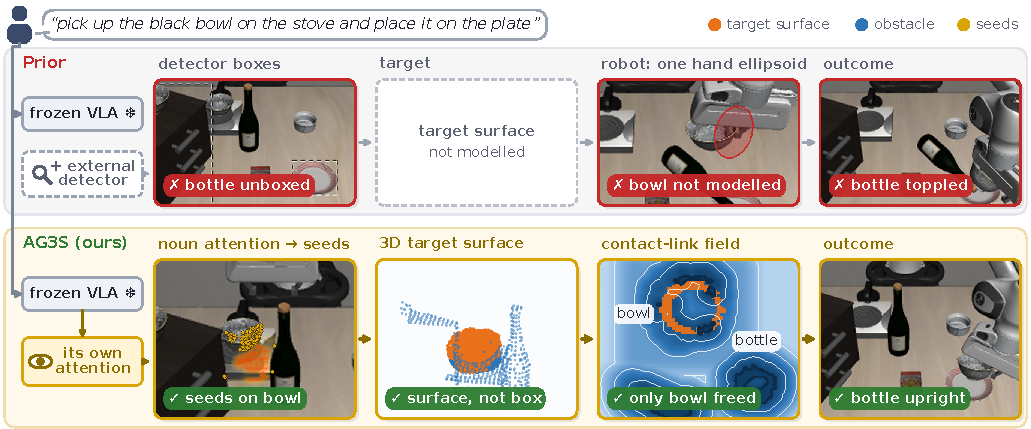
\includegraphics[width=\textwidth]{../figures/fig01_teaser/v5/fig01_v5.pdf}
\caption{\textbf{The policy that is told what to grasp already knows where it is.}
Same SafeLIBERO Level~I episode (initial state and seed) for both lanes; frozen $\pi_{0.5}$, wine bottle as obstacle.
\emph{Prior:} a safety layer needs an add-on open-vocabulary detector; here it boxes the cabinet and the plate but not the bottle, models no target surface, and represents the robot by one end-effector ellipsoid (KNOWS$^\ast$~\cite{park2026knows}), so a carried bowl is unmodelled. AEGIS~\cite{hu2026vlsa} knocks the bottle over, as the policy alone does.
\emph{AG3S:} the same frozen policy's noun attention seeds the bowl (gold); the seeds grow into the bowl's observed 3D surface (orange) while every other observed surface stays an obstacle (blue); the contact links read a distance field from which only that surface is removed (slice at the bowl's height: the bowl is freed, the bottle is not). The bowl is placed and the bottle stays upright.
Camera frames are recorded renders; the 3D and field panels plot the recorded point cloud, voxels, and distance fields of one AG3S planning call.}
\label{fig:teaser}
\end{minipage}
